\documentclass[tikz,border=2pt]{standalone}
\usepackage{fontspec}
\setmainfont{texgyretermes-regular.otf}
\usepackage{pgfplots}
\pgfplotsset{compat=1.18}
\begin{document}
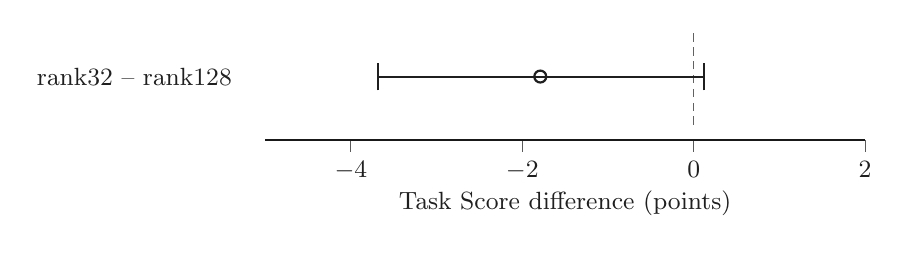
\begin{tikzpicture}
\begin{axis}[
  width=9.2cm,height=3.19cm,
  xmin=-5,xmax=2,ymin=-0.5,ymax=0.5,
  xtick={-4,-2,0,2},
  ytick={},yticklabels={},
  xlabel={Task Score difference (points)},
  axis x line*=bottom,axis y line=none,
  tick align=outside,
  tick style={line width=0.35pt,color=black!65},
  axis line style={line width=0.55pt,color=black!90},
  tick label style={font=\small,color=black!88},
  yticklabel style={font=\small,color=black!88},
  label style={font=\small,color=black!88},
  xlabel style={yshift=1mm},
  yticklabel shift=1mm,
  grid=none,clip=false,
]
\draw[densely dashed,line width=.55pt,color=black!62] (axis cs:0,-0.38) -- (axis cs:0,0.38);
\addplot+[no markers,color=black!88,line width=.7pt] coordinates {(-3.68120096049783,0)(0.118398691152597,0)};
\addplot+[only marks,mark=o,mark size=2.15pt,mark options={color=black!88,fill=white,line width=.8pt}] coordinates {(-1.79062387265512,0)};
\addplot+[no marks,color=black!88,line width=.7pt] coordinates {(-3.68120096049783,-0.11)(-3.68120096049783,0.11)};
\addplot+[no marks,color=black!88,line width=.7pt] coordinates {(0.118398691152597,-0.11)(0.118398691152597,0.11)};
\node[anchor=east,font=\small,text=black!88] at ([xshift=-3mm]axis cs:-5,0) {rank32 -- rank128};
\end{axis}
\end{tikzpicture}
\end{document}
